\section{Auswertung}
\label{sec:Auswertung}

Für die Auswertung wird die Python-Bibliothek \texttt{numpy} benutzt. Die Fits entstehen mit \texttt{curve\_fit} aus \texttt{scipy.optimize}.
Die Fehlerrechnung wird mit \texttt{uncertainties} durchgeführt. Plots entstehen mit \texttt{matplotlib.pyplot}. \\
Vor den Messreihen der beiden Pumpen wird der Rezipient lang genug evakuiert, sodass man einen angenäherten Enddruck $p_\text{E}$ messen kann. \\
Die Evakuierungskurven werden mit mehreren linearen Fits der Form
\begin{equation}
    y = m \cdot x + b
\end{equation}
über die Werte
\begin{equation}
    \ln{\frac{p(t) - p_\text{E}}{p_0 - p_\text{E}}} = -\frac{S}{V}t
    \label{eq:linfit}
\end{equation}
berechnet, sodass die verschiedenen Saugvermögen in den unterschiedlichen Druckbereichen über
\begin{equation}
    S = -m \cdot V
    \label{eq:S_evak}
\end{equation}
berechnet werden können. Dabei ist $m$ die Steigung in $\si{\milli\bar\per\second}$ und $b$ der $y$-Achsenabschnitt in $\si{\milli\bar}$. Im Folgenden werden die Einheiten bei der Angabe dieser Parameter ausgelassen.\\
Bei den Leckratenmessungen wird das Saugvermögen ebenfalls durch einen linearen Fit bestimmt.
$S$ ist hierbei gegeben durch
\begin{equation}
    S = m \cdot \frac{V}{p_\text{G}}
    \label{eq:S_leck}
\end{equation}

\subsection{Drehschieberpumpe}

Der für die Drehschieberpumpe nach einer ungefähr 30 minütigen Mittagspause gemessene Enddruck beträgt
\begin{equation}
    p_\text{E} = (\num{3.83} \pm \num{0.38}) \cdot 10^{-3} \, \si{\milli\bar}.\\
\end{equation}
Das Volumen wird der Versuchsanleitung entnommen und beträgt
\begin{equation}
    V_\text{Drehschieberpumpe} = (\num{34} \pm \num{3.4}) \, \si{\liter}.
\end{equation}


\subsubsection{Evakuierungskurve}

Für die Evakuierungskurve ergibt sich folgender Plot.

\begin{figure}[H]
    \centering
    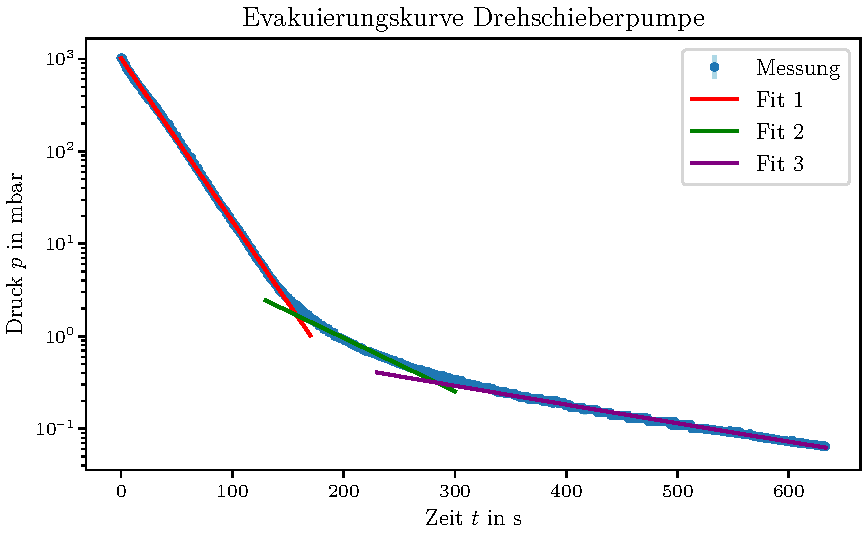
\includegraphics[width=\textwidth]{plots/DP_Evakuierungskurve.pdf}
    \caption{Es werden drei lineare Fits gemacht. Fit 1: $m = \num{-0.0408} \pm \num{0.0007}$, $b = \num{0.01} \pm \num{0.07}$. Fit 2: $m = \num{-0.01441} \pm \num{0.00034}$, $b = \num{-4.16} \pm \num{0.08}$. Fit 3: $m = \num{-0.00597} \pm \num{0.000004}$, $b = \num{-6.174} \pm \num{0.006}$.}
    \label{fig:DP_evak}
\end{figure}

Nach \eqref{eq:S_evak} finde man
\begin{align}
    S_1 &= (\num{1.39} \pm \num{0.14}) \si{\liters\per\second} \\
    S_2 &= (\num{0.49} \pm \num{0.05}) \si{\liters\per\second} \\
    S_3 &= (\num{0.41} \pm \num{0.04}) \si{\liters\per\second} \\
\end{align}